% !TeX spellcheck = en
\documentclass[submission,svgnames,journal=tosc]{iacrtrans}

\usepackage[utf8]{inputenc}
\usepackage{amssymb, amsmath, amsfonts, amscd}
\usepackage[T1]{fontenc}
\usepackage{graphicx}
\usepackage{url}
\usepackage{xspace}
\usepackage{subcaption}
\usepackage{algorithm}
\usepackage{tikz}
\usepackage{minted}
\usepackage{epigraph}
\usepackage{cellspace}
\usepackage{multirow}
\usetikzlibrary{patterns}
\usepackage[noend]{algpseudocode}

\DeclareMathSymbol{:}{\mathord}{operators}{"3A}
\DeclareMathOperator{\LCG}{LCG}
\DeclareMathOperator{\MCG}{MCG}
\DeclareMathOperator{\MAJ}{MAJ}
\DeclareMathOperator{\CVP}{CVP}


% horrible hack
% Math symbol font matha
\DeclareFontFamily{U}{matha}{\hyphenchar\font45}
\DeclareFontShape{U}{matha}{m}{n}{
      <5> <6> <7> <8> <9> <10> gen * matha
      <10.95> matha10 <12> <14.4> <17.28> <20.74> <24.88> matha12
      }{}
\DeclareSymbolFont{matha}{U}{matha}{m}{n}
\DeclareFontSubstitution{U}{matha}{m}{n}

% Math symbol font mathb
\DeclareFontFamily{U}{mathx}{\hyphenchar\font45}
\DeclareFontShape{U}{mathx}{m}{n}{
      <5> <6> <7> <8> <9> <10>
      <10.95> <12> <14.4> <17.28> <20.74> <24.88>
      mathx10
      }{}
\DeclareSymbolFont{mathx}{U}{mathx}{m}{n}
\DeclareFontSubstitution{U}{mathx}{m}{n}

% Symbol definition
\DeclareMathDelimiter{\vvvert}{0}{matha}{"7E}{mathx}{"17}

\newcommand{\todo}[1]{\textcolor{red}{TODO:[#1]}}

\title[Predicting the PCG Pseudo-Random Number Generator in Practice]{Predicting the (non-cryptographic) PCG Pseudo-Random Number Generator In Practice} 

\author{Charles Bouillaguet\inst{1} \and Julia Sauvage\inst{2} \and Florette Martinez\inst{3}}


\institute{% 
University of Lille, France \\ 
\email{charles.bouillaguet@univ-lille.fr}
\and 
Sorbonne University \\
\email{julia.sauvage@etu.upmc.fr}
\and 
LIP6, CNRS, SU ? \\
\email{florette.martinez@lip6.fr}

}

\begin{document}
\maketitle

\keywords{keywords}

\begin{abstract}
  blablabla
\end{abstract}

\section{Introduction} %ce qu'on avait écrit pour le projet, peut-être pas incroyable...

\epigraph{Any one who considers arithmetical methods of producing random digits is, of course, in a state of sin.}{John von Neumann, 1949}

%\todo{Ca, c'est du blabla...}

Pseudo-random generators (PRG) are well-studied primitives in symmetric
cryptography. A PRG is an efficient deterministic algorithm that stretch a small
random seed into a longer pseudo-random stream. To achieve cryptographic-grade
pseudo-randomness, a PRG must ensure that the pseudo-random stream is
computationally indistinguishable from a ``truly'' random sequence of bits by
efficient adversaries. Alternatively, it is possible to define pseudo-randomness
by asking that no efficient algorithm is capable of predicting the next
pseudo-random bit with non-negligible accuracy. The two definitions are in fact
equivalent.

It is well-known that pseudo-random generators can be turned into symmetric
encryption algorithm, by generating ``random'' masks to be used in the one-time
pad. This is precisely what stream ciphers do.

Not all pseudo-random generators are of cryptographic strength. In some
applications, it is not necessarily necessary: to be used in Monte-Carlo
numerical simulations or generate random choices in games, a relaxed,
non-cryptographic notion of pseudo-randomness may be sufficient. This allows for
faster algorithms. For instance, \textsf{python} standard library's
\texttt{random} module uses the Mersenne Twister~\cite{MatsumotoN98}. The
\textsf{C} library that comes along \texttt{gcc} (the \texttt{glibc}) uses a
(poor) truncated linear congruential generator by default to implement the
\texttt{rand} function.

In the realm of non-cryptographic random generators, a PRG is deemed ``good
enough'' it is passes \emph{some} efficient statistical tests --- whereas the
cryptographic notion of pseudo-randomness asks that it passes \emph{any}
efficient test. There are \textit{de facto} statistical test suites; an initial
battery of randomness tests for RNGs was suggested by Knuth in the 1969 first
edition of The Art of Computer Programming. In 1996, Knuth's tests were then
supplanted by Marsaglia's \texttt{Diehard} tests. In 2007, L'Ecuyer proposed
the \texttt{TestU01}~\cite{LEcuyerS07} library, whose ``BigCrush'' test is
considered state-of-the-art by the relevant community, to the best of our
knowledge. In 2010, the NIST proposed its own statistical test suite (Special
Publication 800-22), to which improvements were later
suggested~\cite{ZhuMLZJ16}. We understand that the \texttt{PractRand} test suite
also has a good reputation.

In any case, designers of conventional pseudo-random generators try to obtain
the simplest and fastest algorithm that passes the day's favourite test suite. A
few selected ones are shown in Fig.~\ref{fig:prngs}. \texttt{Lehmer64} is a
truncated linear congruential generator, touted as ``the fastest PRNG that
passes \texttt{BigCrush}''~\cite{LemireLehmer}. \texttt{Xorshift128} is a clever
implementation of a 128-bit LFSR with period $2^{128} - 1$ due to
Marsaglia~\cite{Marsaglia03}, using only a few simple 32-bit
operations. \texttt{Xorshift128+} is a improved version due to
Vigna~\cite{Vigna17} that returns the sum of two consecutive outputs of a
Xorshift LFSR; it passes the ``BigCrush'' test suite and is the default PRNG in
many Javascript implementations, including that in Google's V8 engine (Chrome),
Firefox and Safari.

\begin{figure}
  \begin{minipage}[t]{5cm}
\begin{minted}[fontsize=\small,frame=single]{C}
u128 a;
u64 m = 0xda942042e4dd58b5;

u64_t lehmer64() 
{
    a *= m;
    return a >> 64;
}
\end{minted}
  \end{minipage}
    \begin{minipage}[t]{4cm}
% 128-bit LFSR
\begin{minted}[fontsize=\small,frame=single]{C}
u32 a, b, c, d;


u32 xorshift128()
{
    u32 t = d;
    u32 s = a;
    d = c;
    c = b;
    b = s;
    t ^= t << 11;
    t ^= t >> 8;
    s ^= s >> 19;
    a = t ^ s;
    return a;
}
\end{minted}
    \end{minipage}
    \begin{minipage}[t]{4cm}
    % xorshift128+ (as in google's V8)
\begin{minted}[fontsize=\small,frame=single]{C}
u64 a, b;


u64 xorshift128plus()
{
    u64 s1 = a
    u64 s0 = b;
    a = s0;
    s1 ^= s1 << 23;        
    s1 ^= s1 >> 17;        
    s1 ^= s0;        
    s1 ^= s0 >> 26;
    b = s1;
    return a + b;
}
\end{minted}
    \end{minipage}
    \caption{Some conventional pseudo-random generators, designed for speed and simplicity.}
    \label{fig:prngs}
  \end{figure}
  
Failures in cryptographic pseudo-random generators have catastrophic security
implications. Let us mention for instance the well-known problem in Debian
Linux from 2008, where a bug in the OpenSSL package led to insufficient
entropy gathering and to practical attacks on the SSH and SSL protocols (the
only remaining source of entropy comes from the PID of the process,
\textit{i.e.} 16 bits or less of effective entropy)~\cite{YilekRSES09}.

However, problems in non-cryptographic random number generators can also have
dire consequences (barring the obvious case where they are used in lieu of their
cryptographic counterparts). When they are used in scientific computing for
Monte-Carlo methods, their defects have the potential to alter the results of
numerical simulations. Ferrenberg et al.~\cite{Ferrenberg92} ran a classical
Ferromagnetism Ising model Monte-Carlo simulation, in a special case where the
exact results could be computed analytically, and compared the results of the
simulation with the ``true'' answer. They used several conventional
pseudo-random generators: a 32-bit linear congruential generator, two LFSRs,
various combinations thereof, etc. They observed that changing the source of
random numbers significantly altered the outcome of the numerical
simulation. Different generators produced different biases: in particular a
given LFSRs yielded energy levels that were systematically too low and critical
temperatures that were always too high, while another kind of generator yielded
the opposite (in many, repeated, trials).

The scientific computing community also realized that the need for fast
\emph{parallel} random number generation could be satisfied by the use of block
ciphers in counter mode~\cite{Salmon11}. The need for speed then leads to the
use of weakened cryptographic primitives (round-reduced AES or custom and
presumably weak block-ciphers)

In most cases, it is fairly easy to see that a specific non-cryptographic PRG
does not meet the cryptographic notion of pseudo-randomness, and there are few
exceptions. Most are fairly easy to predict, meaning that after having observed
a prefix of the output, it is easy to produce the next ``pseudo-random''
bits. This makes a good source of exercises for cryptography students.

In this paper, we study the \textsf{PCG} family of non-cryptographic
pseudo-random generators proposed by O'Neil~\cite{melissapaper,melissaweb}. She
did not claim that the algorithm has cryptographic strength, but that predicting
its output ought to be ``challenging''. We therefore took up the challenge.

\textsf{PCG} stands for ``Permuted Congruential Generator'': it essentially
consists in applying a non-linear filtering function on top of a linear
congruential generator (in a way reminiscent to the venerable filtered
LFSRs). The resulting combination is fast and passes current statistical test
suites. The \textsf{PCG} family contains many members, but we focus on the
strongest one, named either \textsf{PCG64} or \textsf{PCG-XSL-RR}. It has a
128-bit internal state and produces 64 bits when clocked. It is the default
pseudo-random number generator in the popular \textsf{NumPy} scientific
computing package for \textsf{Python}.

The internal state of the \textsf{PCG64} generator is made of a 128-bit
``state'' and a 128-bit ``increment'', whose intended use is to provide several
pseudo-random streams with the same seed (just as the initialisation vectors do
in stream ciphers). A default increment is provided in case the end-user just
want one pseudo-random stream with a single 128-bit seed.

\paragraph{Contribution.} We describe an algorithm that reconstructs the full
internal state of the strongest member of the \textsf{PCG} family. This allows
to predict the pseudo-random stream deterministically and clock the generator
backwards. The original seeds can also easily be reconstructed. The state
reconstruction algorithm is practical and we have executed it in practice. It
follows that predicting the output of the \textsf{PCG} should not be considered
challenging anymore.

While the \textsf{PCG} pseudo-random generator is not meant as a cryptographic
primitive, obtaining an actual prediction algorithm requires the use of
cryptanalytic techniques. Making it practical requires in addition a non-trivial
implementation effort.

Our algorithm reconstruct the internal state using a ``guess-and-determine''
approach: some bits of the internal state are guessed ; assuming the guesses are
correct, some other information is computed ; a consistency check discards bad
guesses early on ; then candidate internal states are computed and fully
tested. The problem actually come in two distinct flavors.

When the increment is known (for instance when it is the default value), a
simplified prediction algorithm recovers the internal state from 192 bits of
pseudo-random stream. The process runs in 20 CPU minutes. It guesses 37 bits of
the internal state, then solves an instance of the \textsc{Closest Vector
  Problem} (CVP) in a 3-dimensional euclidean lattice. This requires about 50
arithmetic operations in total and reveals the entire internal state if the
guesses are correct.

When the increment is unknown, things are a bit more complicated. This is the
default situation in \textsf{NumPy}, where both the state and the increment are
initialised using an external source of entropy. In this case, our prediction
algorithm requires 3072 bits of pseudo-random stream ; it guesses between 51 and
55 bits, then for each guess it solves an instance of CVP in dimension 4 (using
about 75 arithmetic operations). This recovers 64 more bits of information about
the difference between two successive states, and this is enough to filter the
bad guesses. This information can then be used in a subsequent and comparably
inexpensive phase to recover the entire internal state. On average, the whole
process requires a bit less than 20 000 CPU hours to complete.

We implemented the algorithms in \textsf{C}, then asked the designer of the PCG
family to send us ``challenge'' pseudo-random streams ; we ran our code and
emailed back the seeds used to generate the challenge streams the next day.

\paragraph{Related Work.} Deterministic pseudo-random generators can be traced
back to the work of Von Neumann and Metropolis on the ENIAC
computer~\cite{vonNeumann1951}; they suggested around 1946 to use the
``middle-square'' method: if $u_n$ is a $k$-digit number, form $u_{n+1}$ by
taking the square of the $\frac{k}{2}$ middle digits of $u_n$. This is a
venerable precursor of the Blum-Blum-Shub ``provably secure'' PRNG. The main
problem of this method is that it produces sequences that quickly enters short
cycles.

Lehmer later proposed linear congruential generators in 1949, also for use on
the ENIAC computer~\cite{Lehmer}. He gave the sequence defined by
$u_0 = 47594118, u_{n+1} = 23 u_n \bmod 10^8 + 1$ and proved that it had period
5882353, a clear improvement compared to the middle-square approach. More
details on early pseudo-random generators can be found in~\cite{Knuth}.

Knuth considered the problem of recovering the internal state of a truncated
linear congruential generator $x_{i+1} = ax_i + c \bmod 2^k$ when $a$ and $c$
are unknown~\cite{Knuth85}; he gave an algorithm exponential in the number of
truncated bits.

The LCG have been largely studied, and considered as cryptographically insecure. 

A reconstruction algorithm has been proposed by D. Knuth in 1985\cite{Knuth85}. The LCG he considered revealed only the upper bits of each internal state. The modulus $2^k$ was known while the multiplier $a$ and the increment $c$ weren't. This algorithm could reconstruct the LCG in $\mathcal{O}(2^l)$ where $l$ is the number of non revealed bit of each internal state.

In 1989, J. Boyar improve the result in a first way \cite{Boyar1989}. She presented an algorithm which could predict a LCG where all the parameters (multiplier, increment and initial state) where unknown under the condition that the number of bit unrevealed was really small in comparison to the modulus.

In 1988, A. Frieze \textit{et al} \cite{Frieze} improve the result in a second way. They supposed that the multiplier $a$ and the modulus $2^k$ were known and used lattice-based technique to recover the LCG more efficiently.

Here we will use techniques presented in \cite{Frieze} to reconstruct some Lehmer's generator (LCG where the increment $c$ is zero) \cite{Lehmer}.

\section{The PCG Pseudo-Random Number Generator Family}

This section introduces some notations and describes the \textsf{PCG64}
non-cryptographic pseudo-random number generator (a.k.a. \textsf{PCG-XSL-RR} in
the designer's terminology).

If $x \in \{0, 1\}^n$ is an $n$-bit string, then $x[i:j]$ denotes the bit string
$x_ix_{i+1}\dots x_{j-2}x_{j-1}$, where $x = x_0\dots x_{n-1}$ (this is the
``slice notation'' used in \textsf{Python}). The set $\mathbb{Z}_{2^k}$ of
integers modulo $2^k$ is seen as the set of $k$-bit strings. If $x$ is a
floating point number, then $\lfloor x \rceil$ denotes the nearest integer
(using the ``rounding half to even'' tie-breaking rule --- this is the default
in IEEE754 arithmetic). If $U$ is a vector or a sequence, then $U_i$ is the
$i$-th element (we use capital letters for these). If $U$ is such a sequence, we
denote by $U \bmod M$ the sequence $(U_0 \bmod M, U_1 \bmod M, \dots)$. The XOR
operation is denoted $\oplus$, left and right rotations are denote $\lll$ and
$\ggg$ respectively. Modular addition is denoted $+$ (or $\boxplus$ to make it
even more explicit).

\textsf{PCG64} has an internal state of 128-bit, which operate as a linear
congruential generator modulo~$2^{128}$. More precisely:
\[
  S_{i+1} = a S_i + c \bmod 2^{128},
\]
Where is a fixed 126-bit constant. The first initial state $S_0$ is the seed of
the generator. The increment $c$ may be specified by the user of the PRNG to
produce different output streams with the same seed (just as the IV acts in a
stream cipher). If no value of $c$ is specified, then a default increment is
provided. Note that $c$ must be odd. The default values are:
\begin{align*}
  a &= \phantom{1}47026247687942121848144207491837523525 & \text{(fixed)}\\
  c &= 117397592171526113268558934119004209487           & \text{(default value, user-definable)}
\end{align*}

Each time the PRNG is clocked, 64 output bits are extracted from the internal
state using a non-linear function that makes use of data-dependent rotations, in
a way reminiscent of the \textsf{RC5} block cipher~\cite{Rivest94}. The six most
significant bits of the internal state encode a number $0 \leq r < 64$. The two
64-bit halves of the internal state are XORed together, and this 64-bit result
is rotated right by $r$ positions.

The successive 64-bit outputs of the generator are $X_0, X_1, \dots$ where:
\begin{equation}\label{eq:output}
  X_i =(\underbrace{S_i[0:64] \oplus S_i[64:128]}_{Y_i}) \ggg \underbrace{S_i[122:128]}_{r_i}.
\end{equation}
For the sake of convenience, we denote by $Y_i$ the XOR of the two halves of the
state (before the rotation) and by $r_i$ the number of shifts of the ``$i$-th
rotation''.

Fig.~\ref{pcg128out} summaries the process. The overall design strategy is
similar to that of a filtered LFSR: the successive states of a weak internal
generator with a strong algebraic structure are ``filtered'' by a non-linear
function.

Updating the internal state requires a $128 \times 128 \rightarrow 128$
multiplication operation. In fact, this can be done with three
$64 \times 64 \rightarrow 128$ multiplication and two 64-bit additions. High-end
desktop CPUs all implement these operations in hardware, so the generator is
quite fast on these platforms.


\begin{figure}
  \begin{center}
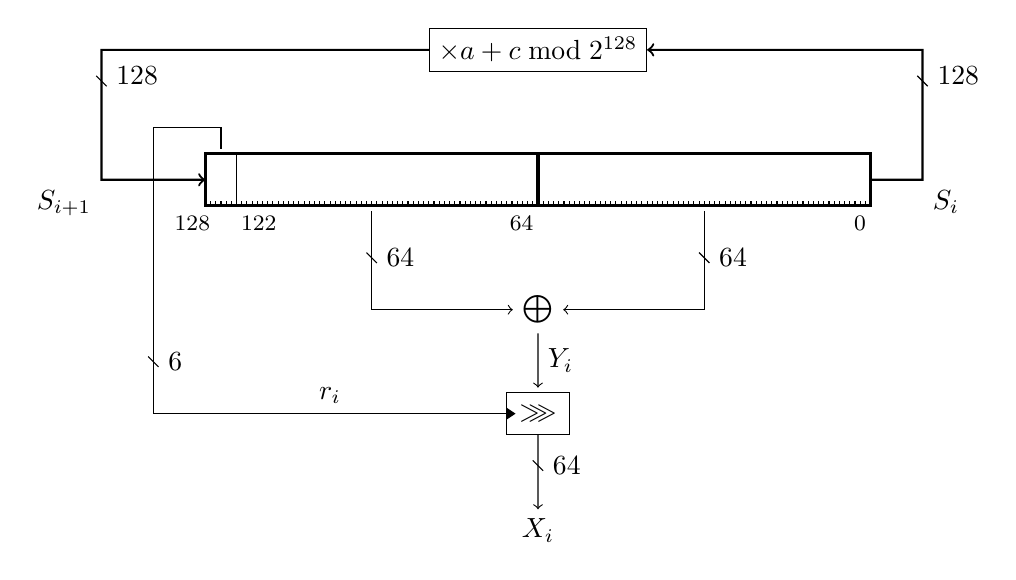
\begin{tikzpicture}[scale=0.66]
%  \draw[red, use as bounding box] (-1.25, -6.75) rectangle (12.8, 2.25);
  
  % S_i

    % bordures
    \draw[very thick]  (0, 0) rectangle (12.8, 1);
    \draw  (0.6, 0) rectangle +(0, 1);
    \draw[very thick]  (6.4, 0) rectangle +(0, 1);
    \foreach \i in {0, 1, ..., 128} \draw (\i/10, 0) -- +(0, 0.1);
    
    % déco autour
    \node[draw] at (6.4, 3) (update) {$\times a + c \bmod 2^{128}$};
    \draw[thick,->] (12.8, 0.5) -- (13.8, 0.5) node[below right] {$S_i$} -- (13.8, 3) -- (update);
    \draw (13.7, 2.5) -- +(0.2, -0.2);
    \path (13.9, 2.5) node[anchor=west] {128};

    \draw[thick,->] (update) -- (-2, 3) -- (-2, 0.5) node[below left] {$S_{i+1}$} -- (0, 0.5);
    \draw (-2.1, 2.5) -- +(0.2, -0.2);
    \path (-1.9, 2.5) node[anchor=west] {128};

    
    \node[font=\footnotesize,anchor=east] at (12.9, -0.33) {0};
    \node[font=\footnotesize,anchor=east] at (6.5, -0.33) {64};
    \node[font=\footnotesize,anchor=west] at (0.5, -0.33) {122};
    \node[font=\footnotesize] at (-0.25, -0.33) {128};
    
    \draw (6.4, -2) node (x) {$\bigoplus$};
    
    \draw[->] (3.2, -0.1) |- (x);
    \draw (3.1, -0.9) -- +(0.2, -0.2);
    \path (3.3, -1) node[anchor=west] {64};
    
    \draw[->] (9.6, -0.1) |- (x);
    \draw (9.5, -0.9) -- +(0.2, -0.2);
    \path (9.7, -1) node[anchor=west] {64};

    \node[minimum width=1.8cm] at (6.4, -4) (r) {$\ggg$};
    \draw (5.8, -3.6) rectangle +(1.2, -0.8);
    \draw[fill=black] (5.8, -4.1) -- (5.95, -4) -- (5.8, -3.9) -- cycle;
    
    \draw (0.3, 1.1) -- (0.3, 1.5) -- (-1, 1.5) -- (-1, -4) -- node[above] {$r_i$} (5.8, -4);
    \draw (-1.1, -2.9) -- +(0.2, -0.2);
    \path (-0.9, -3) node[anchor=west] {6};

    \draw[->] (x) -- node[right] {$Y_i$} +(0, -1.5);
    \node at (6.4, -6.25) (xi) {$X_i$};
    \draw[->] (6.4, -4.4) -- (xi);

    \draw (6.3, -4.9) -- +(0.2, -0.2);
    \path (6.5, -5) node[anchor=west] {64};
  \end{tikzpicture}
\end{center}
\caption{\textsf{PCG64}: Internal state update and output process.}
\label{pcg128out}
\end{figure}


\section{Tools}
\label{sec:geometric}

In the rest of this paper, we often perform arithmetic operations on integers
where only some bits are known. This leads to generation of unknown carries. If
$a, b$ are integers modulo $2^{128}$ and $0\leq i<j<128$, then there is a
\emph{carry} $0 \leq \gamma \leq 1$ (resp. a \emph{borrow}
$0 \leq 1 \leq \beta$) such that:
\begin{align}
  (a \boxplus b)[i:j]  &= a[i:j] \boxplus  b[i:j] \boxplus  \gamma, \label{eq:caryy}  \\
  (a \boxminus b)[i:j] &= a[i:j] \boxminus b[i:j] \boxminus \beta.  \label{eq:borrow}
\end{align}

\subsection{Linear Congruential Generators and Lattices}

Given an integer $k$, a fixed multiplier $a$, an increment $c$ and a ``seed''
$x$, define the sequence:
\[
  U_0 = x, U_{i+1} = a U_i + c.
\]
When reduced modulo $2^k$, the sequence $U$ form the successive states of a
linear congruential generator (LCG). Let $\LCG_{k}(x, c)$ denote the vector
$(u_0, u_1, u_2, \dots)$ of integers modulo $2^k$. It is easy to check that:
\begin{align}
\label{eq:lcg-additive}
\LCG_{k}(x + y, c + d) &= \LCG_{k}(x, c) + \LCG_{k}(y, d),  \\
\label{eq:lcg-scalar}
\LCG_{k}(\lambda x, \lambda c) &= \lambda \LCG_{k}(x, c).   
\end{align}

Let $\mathcal{L}$ denote the euclidean lattice spawned by the rows of the
following $n\times n$ matrix:
\[
  G_{n,k} = \begin{pmatrix}
    1 & a   & a^2 & \dots & a^{n-1} \\
    0 & 2^k & 0   & \dots & 0 \\
    0 & 0   & 2^k & \dots & 0 \\
    \dots & \dots & \dots & \dots & \dots\\
    0 & 0 & 0 & \dots & 2^k \\
  \end{pmatrix}
\]
This lattice contains all $n$-terms geometric progressions of common ratio $a$
modulo $2^k$; therefore the first $n$ terms of the sequence $\LCG_{k}(x, 0)$
give the coordinates of a point of this lattice.

Reconstructing the state of a truncated linear congruential generator can
generally be seen as the problem of finding a point of this lattice given only
an approximation thereof, for instance when the least-significant bits of each
components have been dropped. The ``lattice approach'' to truncated linear
congruential generators is due to Frieze \textit{et al.}~\cite{Frieze}.

Let $U$ be a vector of $n$ integers modulo $2^k$ such that
$U_{i+1} = a U_i \bmod 2^k$; it is a geometric progression of common ratio $a$,
modulo $2^k$, therefore $(U_0, \dots, U_{n-1}) \in \mathcal{L}$. Let
$T_i = U_i[k-\ell:k]$ denote the top $\ell$ bits of $U_i$, and let $N$ denote an
arbitrary ``noise vector'' such that $N_i \in \{-1, 0, 1\}$. Finally, set
$\widetilde{T}_i = T_i + N_i \bmod 2^{\ell}$.  We will be facing the following
problem (``reconstructing noisy truncated geometric series'') several times:
\begin{description}
\item[INPUT]  $\widetilde{T} = (\widetilde{T}_0, \dots, \widetilde{T}_{n-1}) \in \left(\mathbb{Z}_{2^\ell}\right)^n$, a (noisy) version of $U$ truncated to the top $\ell$ bits.
\item[OUTPUT] $U_0 \bmod 2^k$, the first term of the (non-truncated) geometric sequence.
\end{description}

We will be facing a ``high-dimension'' instance in section~\ref{sec:big_cvp}
and many ``low-dimension'' in sections~\ref{sec:Cknown}
and~\ref{sec:Cunknown}. The rest of this section discusses algorithmic tools to
solve these problems. We first claim that $2^{k-\ell} \widetilde{T}$ is
``close'' to a point of the lattice $\mathcal{L}_{n,k}$.

\begin{lemma}\label{thm:close}
  There exists $U' \in \mathcal{L}$ such that $U'_i \equiv U_i \bmod 2^k$
  and $\left\lVert U' -2^{k-\ell} \widetilde{T} \right\rVert \leq 2 \sqrt{n} 2^{k-\ell}$.
\end{lemma}


\begin{proof}
  We first observe that $U$ belongs to the lattice $\mathcal{L}$. We start by setting $U' \gets U$, and we examine all coordinates of $U$:
  \begin{itemize}
  \item If $\widetilde{T}_i = T_i + N_i$ (without modulo), then we have:
    \begin{align*}
      \left| 2^{k-\ell}\widetilde{T}_i-U_i \right| &= \left| 2^{k-\ell}(T_i + N_i)-U_i \right| 
                                                     = \left| 2^{k-\ell}N_i - U_i[0,k-\ell] \right| \\
                                                   &\leq \left| 2^{k-\ell}N_i\rvert + \lvert U_i[0,k-\ell] \right| 
                                                   % &\leq 2^{k-\ell} + 2^{k-\ell} - 1\\
      \leq 2^{k-\ell +1 }.
    \end{align*}
    
  \item Otherwise, there are two possible ``wraparound'' cases:
    \begin{itemize}
    \item Either $T_i = 0$ and $N_i = -1$, which leads to $\widetilde{T}_i = 2^\ell-1$. 
      In this case, we have $U_i = U_i[0,k-\ell]$ and we set $U'_i = U_i + 2^{k}$ (note that this amount to adding a lattice vector to $U'$, so $U'$ stays in the lattice). We have:
      \[
        \left| 2^{k-\ell}\widetilde{T}_i-(U_i + 2^k) \right| = %\left| 2^{k-\ell}(2^\ell -1) -(U_i + 2^k) \right| =
        \left| 2^{k-\ell} + U_i[0,k-\ell]\right| \leq 2^{k-\ell + 1}. 
      \]
      
    \item Or $T_i = 2^{\ell}-1$ and $N_i = +1$, which leads to
      $\widetilde{T}_i = 0$.  This implies that
      $U_i= 2^k-2^{k-\ell} + U_i[0,k-\ell]$; we set $U'_i = U_i - 2^k$ (again,
      with this modification $U'$ stays in the lattice), and we find:
      \[
        \left| 2^{k-\ell}\widetilde{T}_i-(U_i - 2^k) \right| %=\left| 0 -(U_i - 2^k) \right|
        = \left| 2^k-2^{k-\ell} + U_i[0,k-\ell] - 2^k\right| \leq 2^{k-\ell + 1}.
      \]
    \end{itemize}
  \end{itemize}
  In the end, we have
  $\left\| U' -2^{k-\ell} \widetilde{T} \right\| \leq 2 \sqrt{n} 2^{k-\ell}$,
  and $U' \equiv U \mod 2^k $.
\end{proof}

\subsection{Reconstruction in ``High'' Dimension Using an Exact CVP Solver}

Lemma~\ref{thm:close} tells us that the approximation of a geometric sequence
obtained by dropping least-significant bits cannot be arbitrarily far from a
lattice point which reveals $U_0 \bmod 2^k$. Therefore, we may possibly
reconstruct truncated geometric series by finding the lattice vector closest to
the approximation we have. This means solving instances of the well-known
\textsf{Closest Vector Problem} (CVP), a fundamental hard problem on
lattices. It is NP-hard, and all known algorithms are exponential in the
dimension of the lattice, yet they can be fairly practical up to dimension
$\approx 70$.

Let $\CVP(\mathcal{L}, x)$ denote the vector of $\mathcal{L}$ closest to the
input vector $x$. Using the same notations as above, we want to know if
$\CVP\left(\mathcal{L}, 2^{k-\ell}\widetilde{T}\right)$ is indeed $U'$. This
will necessarily be the case when $\|2^{k-\ell}\widetilde{T} - U'\|$ is smaller
than the length of the shortest non-zero vector of $\mathcal{L}$ --- this quantity,
the \emph{first minimum} of the lattice, is denoted by $\lambda_1(\mathcal{L})$.
%What can we say about $|CVP(L,2^{k-\ell}\widetilde{T})-U'|$ ?
By the triangular inequality, we have:
\begin{align*}
|\CVP(\mathcal{L}, T) - U'| %&= \left| \CVP\left( \mathcal{L}, 2^{k-\ell}\widetilde{T} \right) \riht| + \left|2^{k-\ell}\widetilde{T} - U'\right| %-2^{k-\ell}\widetilde{T}+2^{k-\ell}\widetilde{T}-U'|\\
                             & \leq \left| \CVP\left(\mathcal{L}, 2^{k-\ell}\widetilde{T} \right) - 2^{k-\ell}\widetilde{T}\right | + \left|2^{k-\ell}\widetilde{T} - U'\right|.
\end{align*}
But, as the vector $U'$ belongs to the lattice, by definition of the closest
vector and by lemma~\ref{thm:close}:
% $|CVP(L,2^{k-\ell}\widetilde{T})-2^{k-\ell}\widetilde{T}| \leq
% |2^{k-\ell}\widetilde{T}-U'| $, hence
\[
  |\CVP(\mathcal{L}, T) - U'| \leq 2 \left|2^{k-\ell} \widetilde{T} - U' \right| \leq 4 \sqrt{n} 2^{k-\ell}.
\]

If we can prove that the right side of this inequality is smaller than the first
minimum of the lattice $\lambda_1(\mathcal{L})$, then we would have proved that
$\CVP(\mathcal{L}, T)$ indeed reveals $U_0 \bmod 2^k$.

In section~\ref{sec:big_cvp}, we will be facing the problem of reconstructing a
geometric sequence modulo $2^{128}$ given arbitrarily many (noisy versions of
the) most-significant $6$ bits of successive elements of the sequence. Therefore
we have $k=128$ and $\ell=6$, and we wish to determine the required number of
samples, \textit{i.e.} the value of $n$. This means finding the values of $n$
such that $\sqrt{n} 2^{124} \leq \lambda_1\left(\mathcal{L}\right)$.

Starting from $n=\lceil 122/6\rceil\rceil$, we computed the length of the
shortest vector of the lattice spanned by $G_{n, 128}$ for each successive $n$
until the condition holds. The \textsf{Shortest Vector Problem} is another
well-known lattice NP-hard problem; we used the (almost) off-the-shelf
\texttt{G6K} library~\cite{AlbrechtDHKPS19}, which gave results very quickly by
sieving. \texttt{fplll}~\cite{fplll} was too slow above dimension 50, in the
default settings.

After this computation, we found that the minimal possible $n$ is 63: with
$n=63$, the shortest vector of $\mathcal{L}$ has length greater than
$2^{127.02}$, which is high enough. This vector can be obtained by bootstrapping
the geometric sequence with
\[
  U_0 = 12144252875850345479015002205241987363
\]
then reducing the terms modulo $2^{128}$ in zero-centered representation
(subtracting $2^{128}$ to $U_i$ if $U_i > 2^{127}$). It follows that when
$n\geq 63, k=128$ and $\ell=6$, any CVP oracle will return a vector congruent to
the original $U$ when given $\widetilde{T}$.



\subsection{Reconstruction in Low Dimension Using Babai's Rounding}

In sections~\ref{sec:Cknown} and~\ref{sec:cvp_small_2} we will need to
reconstruct billions of noisy truncated geometric series modulo $2^{64}$ with
very few terms, of which a large fraction of most-significant bits are known. In
this setting, the CVP problem becomes much easier. This enables us to use faster
and more \textit{ad hoc} methods, such as Babai's rounding
algorithm~\cite{Babai86}.

If $M$ is a square matrix, we denote by $\vvvert M \vvvert$ the induced matrix norm :
\[
  \vvvert M \vvvert =  \sup_{x \in \mathbb{R}^n} \frac{\| xM \|}{\| x \|}
\]
In the case of the $\| \cdot \|_2$ norm used throughout this paper, $\| M \|$ is
the largest singular value of $G$; equivalently, it is the square root of the
absolute value of the largest eigenvalue of $M^{t} M$.

Denote again by $\mathcal{L}$ the $n$-dimensional lattice spanned by the rows of
$G_{n,64}$, and let $H$ denote the LLL-reduction of $G_{n,64}$. The same lattice
is also spanned by the rows of $H$. For instance, with $n=3$:
\[
  H = \left(\begin{array}{rrr}
                -1241281756092 & 3827459685972 & -728312298332 \\
                -5001120657083 & -2117155768935 & 5479732607037 \\
                8655886039732 & 3303731088004 & 6319848582548
              \end{array}\right)
\]
Set $S = 2^{k-\ell} \widetilde{T}H^{-1}$; as $2^{k-\ell}\widetilde{T}$ is not
\textit{a priori} an element of the lattice, $S$ need not be an integer
vector. Let then $R$ denote the rounding of $S$, \textit{i.e.}
$R_i = \left\lfloor S_i \right\rceil$. Then $R H$ is an element of the
lattice. Under the right conditions, it will be the vector of the lattice
closest to $2^{k-\ell} \widetilde{T}$. Indeed:
\begin{align*}
\lVert U' - R H \rVert &= \left\| U' - \left(R - 2^{k-\ell}\widetilde{T}H^{-1} + 2^{k-\ell}\widetilde{T}H^{-1}\right)H \right\| \\
&= \left\| U' - 2^{k-\ell}\widetilde{T} - \left(R - 2^{k-\ell} \widetilde{T}H^{-1}\right )H \right\| \\
&\leq \left\| U' - 2^{k-\ell}\widetilde{T} \right\| + \left\| R - 2^{k-\ell}\widetilde{T}H^{-1} \right\| \times \vvvert H \vvvert.
\end{align*}
By definition, $R$ is the closest integer vector to
$2^{k-\ell}\widetilde{T}H^{-1}$. But as $U'$ is an element of the lattice,
$U'H^{-1}$ is an integer vector. Thus $R-2^{k-\ell}\widetilde{T}G^{-1}$ is
shorter than $U'G^{-1}-2^{k-\ell}\widetilde{T}G^{-1}$. Hence :
\begin{align*}
  \left\| U' - RH \right\| &\leq \left\| U' - 2^{k-\ell}\widetilde{T} \right\| + \left\|R - 2^{k-\ell}\widetilde{T}H^{-1}\right\| \times \vvvert H \vvvert \\	
                        &\leq \left\| U' - 2^{k-\ell}\widetilde{T} \right\| + \left\|U'H^{-1}-2^{k-\ell}\widetilde{T}H^{-1}\right\| \times \vvvert H \vvvert \\	
                        &\leq \left\| U' - 2^{k-\ell}\widetilde{T} \right\| + \left\|U' - 2^{k-\ell}\widetilde{T}\right\| \times \left\vvvert H^{-1} \right\vvvert  \times \vvvert H \vvvert \\
                        & 	\leq \left\| U' - 2^{k-\ell}\widetilde{T} \right\| \times \left(1 + \vvvert H^{-1} \vvvert  \times \vvvert H \vvvert \right).
\end{align*}

If we can prove that the right side of the inequality is smaller than the first
minimum of the lattice, then we would have proved that $RH$ is indeed the
closest vector we were searching for. Because we have fixed $k = 64$, by
lemma~\ref{thm:close} we have
$\left\| 2^{k-\ell}\widetilde{T} - U' \right\| \leq 2 \sqrt{n}2^{64-\ell}-1
$. So, if we fix $n$ we can search for the minimum number $\ell$ of known
most-significant bits such that:
\[
  \left(1 + \vvvert H \vvvert \times \left\vvvert H^{-1} \right\vvvert \right) 2 \sqrt{n} 2^{64-\ell} \leq \lambda_1(\mathcal{L})
\]

\begin{table}[htbp!]
  \centering
  \begin{tabular}{|c|Sc|Sc|c|}
	\hline
	n & $\vvvert H \vvvert \times \left\vvvert H^{-1} \right\vvvert$ & $ \lambda_1(\mathcal{L}) $ & minimum $\ell$ \\
	\hline
	3 & 2.87 & $4.09e^{12} \simeq 2^{41.9}$ & 26 \\
	4 & 2.06 & $2.44e^{14} \simeq 2^{47.8}$ & 20 \\
	5 & 3.77 & $1.72e^{15}\simeq 2^{50.6}$ & 18 \\
	6 & 2.69 & $1.03e^{16}\simeq 2^{53.2}$ & 15 \\
	\hline
  \end{tabular}
  \caption{minimal $\ell$ needed for a given $n$}
  \label{tab:babai}
\end{table}

When $\ell$ is greater than the values given in table~\ref{tab:babai}, then
Babai's rounding technique will always return the closest vector, and allow us
to reconstruct a truncated geometric series.

\subsection{Application to the \texttt{Lehmer64} generator}

Adapting the previous reasoning enables an efficient state reconstruction
algorithm for the \texttt{Lehmer64} generator shown in
Fig.~\ref{fig:prngs}. When clocked, it outputs the top 64 bits of a geometric
sequence ($k=128$ and $\ell=64$). Three successive outputs are sufficient to
reconstruct the internal state using Babai's rounding technique. This yields the
following reconstruction algorithm:
\begin{minted}[fontsize=\scriptsize]{python}
def reconstruct(X):
    """
    Produce the internal state of the generator given three consecutive outputs.
    16 multiplications, 1 division, 11 additions and 3 roundings only.
    """
    a = 0xda942042e4dd58b5
    r = round(2.64929081169728e-7 * X[0] + 3.51729342107376e-7 * X[1] + 3.89110109147656e-8 * X[2])
    s = round(3.12752538137199e-7 * X[0] - 1.00664345453760e-7 * X[1] - 2.16685184476959e-7 * X[2])
    t = round(3.54263598631140e-8 * X[0] - 2.05535734808162e-7 * X[1] + 2.73269247090513e-7 * X[2])
    u = r * 1556524 + s * 2249380 + t * 1561981
    v = r * 8429177212358078682 + s * 4111469003616164778 + t * 3562247178301810180
    state = (a*u + v) % (2**128)
    return state
\end{minted}

But enough fooling around. Let's go back to \textsf{PCG64}.

\section{State Reconstruction for \textsf{PCG64} With Known Increment}
\label{sec:Cknown}

We first consider the easier case where the ``increment'' (the $c$ term in the
definition of the underlying linear congruential generator) is known --- recall
that a default value is specified in case the user of the pseudo-random
generator does not want to provide one.

In this case, reconstructing the 128-bit internal state $S_i$ of the generator
is sufficient to produce the pseudo-random flow with 100\% accuracy (the
generator can also be clocked backwards if necessary, so that the seed can be
easily reconstructed). We therefore focus on reconstructing $S_0$ (the seed)
from $X_0, X_1, X_2, \dots$. A very simple strategy could be the following:
\begin{enumerate}
\item Guess the 64 upper bits of $S_0$ (this includes the rotation).
\item Compute the missing 64 lower bits using~\eqref{eq:output}, with:
\[
   S_0[0:64] = S_0[64:128] \oplus (X_0  \lll S[122:128]).
\]
\item Compute $S_1$ then extract $X_1$; if $X_1$ is correct, then output $S_0$.
\end{enumerate}

This ``baseline'' procedure requires $2^{64}$ iterations of a loop that does a
dozen arithmetic operations; it always output the correct value of $S_0$, and
may output a few other ones (they can be easily discarded by checking $X_2$). An
improved ``guess-and-determine'' state reconstruction algorithm is possible,
which essentially amounts to expose a truncated version of the underlying linear
congruential generator, and attack it using the tools exposed in
section~\ref{sec:geometric}. This is possible by combining the following
ingredients:
\begin{itemize}
\item The underlying linear congruential generator uses a power-of-two modulus,
  therefore the $\ell$ low-order bits of $S_{i+1}$ are entirely determined by
  the $\ell$ low-order bits of $S_i$. More precisely, we have:
  \begin{equation}\label{eq:lcg}
    S_{i+1} = aS_i + c \bmod 2^\ell, \qquad \text{for all } 0 \leq \ell \leq 128
  \end{equation}
  Therefore, guessing the least-significant bits of $S_0$ yields a ``long-term
  advantage'' that holds for all subsequent states.

\item Guessing a 6-bit rotation $r_i$ gives access to $Y_i$ (the XOR of the two
  halves of the internal state). Thus, if a part of the state is known, then
  this transfers existing knowledge to the other half.
\end{itemize}

In figure~\ref{fig:Cknown}, we see that guessing $S_0[0:\ell]$ and a few 6-bit
rotations $r_i$ give access to $S_i[58:64+\ell]$ for the corresponding
states. Therefore, looking at $S_i[\ell:64+\ell]$, we are facing a truncated
linear congruential generator on $64$ bits, where we have access to the most
$6+\ell$ bits of each state (denoted by $T$), for a few consecutive states. This
is sufficient to reconstruct entirely the successive states of this truncated
linear congruential generator. This reveals $S_0[\ell:64+\ell]$, and
using~\eqref{eq:output} the entire $S_0$ can be reconstructed. The precise
details follow.

\begin{figure}
\begin{center}
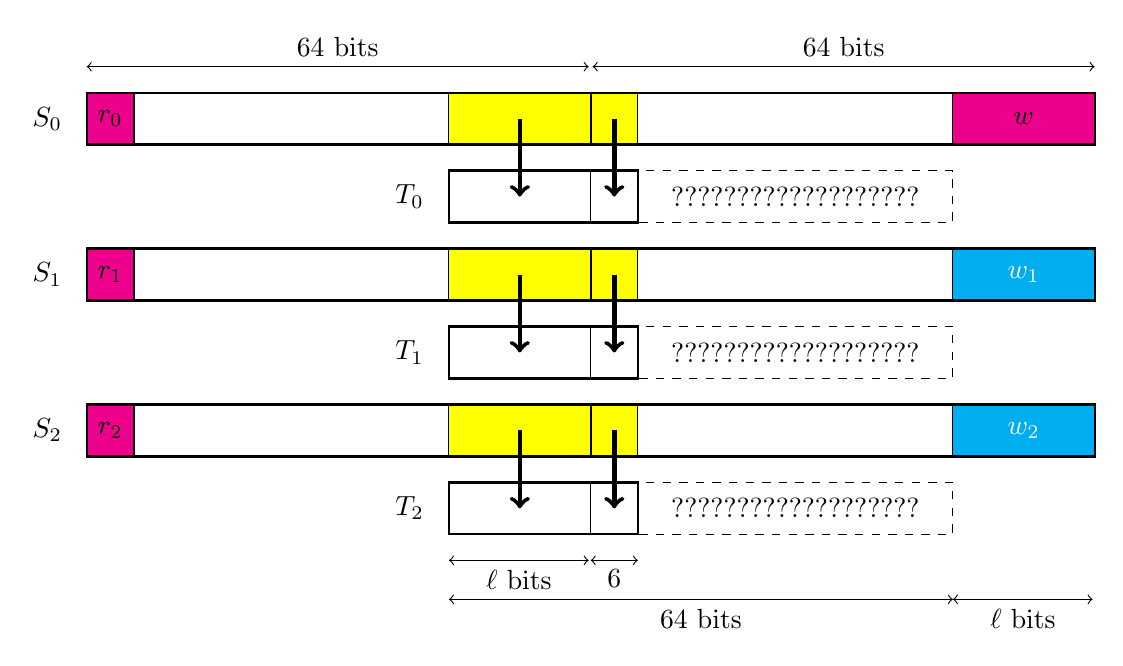
\begin{tikzpicture}[yscale=0.66]
  \path[red, use as bounding box] (-0.75, -9.5) rectangle (12.8, 2.25);
  
  % S_0
  \begin{scope}
    % remplissage
    \fill[fill=Yellow] (4.6, 0) rectangle +(2.4, 1);
    \fill[fill=magenta] (0, 0) rectangle node {$r_0$} +(0.6, 1);
    \fill[fill=magenta] (11, 0) rectangle node {$w$} +(1.8, 1);
    
    % bordures
    \draw[thick]  (0, 0) rectangle (12.8, 1);
    \draw  (0.6, 0) rectangle +(0, 1);
    \draw[thick]  (6.4, 0) rectangle +(0, 1);
    \draw  (7.0, 0) rectangle +(0, 1);
    \draw  (4.6, 0) rectangle +(0, 1);
    \draw  (11, 0) rectangle +(0, 1);
    
    % déco autour
    \node at (-0.5, 0.5) {$S_0$};
    \draw[<->] (0, 1.5) -- node[above] {64 bits} +(6.375, 0);
    \draw[<->] (6.425, 1.5) -- node[above] {64 bits} +(6.375, 0);
  \end{scope}

  % T_0
  \begin{scope}[xshift=4.6cm, yshift=-1.5cm]    
    \draw[dashed]  (0, 0) rectangle +(6.4, 1);
    \draw[thick]  (0, 0) rectangle +(2.4, 1);
    \draw[]  (1.8, 0) rectangle +(0, 1);
    \path (2.4, 0) rectangle node {$???????????????????$} (6.4, 1);

    % déco
    \node at (-0.5, 0.5) {$T_0$};
  \end{scope}

  % flèches S_i --> T_i
  \draw[ultra thick,->] (5.5, 0.5) -- +(0, -1.5);
  \draw[ultra thick,->] (6.7, 0.5) -- +(0, -1.5);

  
  %%%%%%%%%

  
  % S_1
  \begin{scope}[yshift=-3cm]
    % remplissage
    \fill[fill=Yellow] (4.6, 0) rectangle +(2.4, 1);
    \fill[fill=magenta] (0, 0) rectangle node {$r_1$} +(0.6, 1);
    \fill[fill=cyan] (11, 0) rectangle node[text=white] {$w_1$} +(1.8, 1);
    
    % bordures
    \draw[thick]  (0, 0) rectangle (12.8, 1);
    \draw  (0.6, 0) rectangle +(0, 1);
    \draw[thick]  (6.4, 0) rectangle +(0, 1);
    \draw  (7.0, 0) rectangle +(0, 1);
    \draw  (4.6, 0) rectangle +(0, 1);
    \draw  (11, 0) rectangle +(0, 1);
    
    % déco autour
    \node at (-0.5, 0.5) {$S_1$};

    % flèches S_i --> T_i
    \draw[ultra thick,->] (5.5, 0.5) -- +(0, -1.5);
    \draw[ultra thick,->] (6.7, 0.5) -- +(0, -1.5);
  \end{scope}

  % T_1
  \begin{scope}[xshift=4.6cm, yshift=-4.5cm]    
    \draw[dashed]  (0, 0) rectangle +(6.4, 1);
    \draw[thick]  (0, 0) rectangle +(2.4, 1);
    \draw[]  (1.8, 0) rectangle +(0, 1);
    \path (2.4, 0) rectangle node {$???????????????????$} (6.4, 1);

    % déco
    \node at (-0.5, 0.5) {$T_1$};
  \end{scope}

  %%%%%%%%%%%%%

  
  % S_2
  \begin{scope}[yshift=-6cm]
    % remplissage
    \fill[fill=Yellow] (4.6, 0) rectangle +(2.4, 1);
    \fill[fill=magenta] (0, 0) rectangle node {$r_2$} +(0.6, 1);
    \fill[fill=cyan] (11, 0) rectangle node[text=white] {$w_2$} +(1.8, 1);
    
    % bordures
    \draw[thick]  (0, 0) rectangle (12.8, 1);
    \draw  (0.6, 0) rectangle +(0, 1);
    \draw[thick]  (6.4, 0) rectangle +(0, 1);
    \draw  (7.0, 0) rectangle +(0, 1);
    \draw  (4.6, 0) rectangle +(0, 1);
    \draw  (11, 0) rectangle +(0, 1);
    
    % déco autour
    \node at (-0.5, 0.5) {$S_2$};
    
    % flèches S_i --> T_i
    \draw[ultra thick,->] (5.5, 0.5) -- +(0, -1.5);
    \draw[ultra thick,->] (6.7, 0.5) -- +(0, -1.5);
  \end{scope}

  % T_2
  \begin{scope}[xshift=4.6cm, yshift=-7.5cm]    
    \draw[dashed]  (0, 0) rectangle +(6.4, 1);
    \draw[thick]  (0, 0) rectangle +(2.4, 1);
    \draw[]  (1.8, 0) rectangle +(0, 1);
    \path (2.4, 0) rectangle node {$???????????????????$} (6.4, 1);

    % déco
    \node at (-0.5, 0.5) {$T_2$};
    \draw[<->] (0, -0.5) -- node[below] {$\ell$ bits} +(1.775, 0);
    \draw[<->] (1.8, -0.5) -- node[below] {6} +(0.6, 0);
    \draw[<->] (0, -1.25) -- node[below] {64 bits} +(6.4, 0);
    \draw[<->] (6.4, -1.25) -- node[below] {$\ell$ bits} +(1.775, 0);
  \end{scope}
\end{tikzpicture}

\end{center}
\caption{A guess-and-determine algorithm to reconstruct the first internal state
  $S_0$. Magenta bits are guessed; cyan bits are obtained using the linear
  congruence relation~\eqref{eq:lcg} modulo $2^\ell$; yellow bits are obtained
  from the output and the guessed rotations using~\eqref{eq:output}.}
\label{fig:Cknown}
\end{figure}

We consider the sequence of internal states
$S = (S_0, S_1, \dots) = \LCG_{128}(S_0, c)$. We will guess the $\ell$
least-significant bits of $S_0$, therefore let us assume that their value is
known and denote it by $w$. We define $S' = \LCG_{128}(S_0 - w, 0)$ and
$K = \LCG_{128}(w, c)$ --- this is Known. By~\eqref{eq:lcg-additive}, we have
$S' = S - K$. The point is that the elements of $S'$ follow a geometric
progression of common ratio $a$; in addition, the $\ell$ least significant bits
of each components are equal to zero. It follows that $S'[\ell:64+\ell]$ also
follows a geometric progression of common ratio $a$, this time modulo
$2^{64}$. The crux of the reconstruction algorithm is to find
$S'[\ell:64+\ell]$.

We know $K_i[58:64+\ell]$ for all $i$, and for each guessed rotation $r_i$ we
have access to $T_i \stackrel{def}{=} S_i[58:64+\ell]$.  We want
$T'_i \stackrel{def}{=} (S_i \boxminus K_i)[58:64+\ell]$, which is the
truncation of $S'_i$. Thanks to~\eqref{eq:borrow}, we know that there is an
unknown vector $B$ of \emph{borrows}, whose components are either 0 or 1, such
that $T' = S[58:64+\ell] \boxminus K[58:64+\ell] \boxminus B$. Because the
borrows are unknown, we in fact compute
$\widetilde{T'} = S[58:64+\ell] \boxminus K[58:64+\ell]$, and clearly
$\widetilde{T'} = T' \boxplus B$. We are thus in the context of the problem
discussed in section~\ref{sec:geometric}, namely reconstructing a geometric
sequence given $6+\ell$ (noisy) most-significant bits. The ``noise'' is the
unknown vector $B$ of borrows.

We will guess $n$ rotations and $\ell$ least-significant bits of the state, for
a total of $2^{6n + \ell}$ guessed bits. Table~\ref{tab:babai} gives a
lower-bound on $\ell$ given $n$, and we see that the total number of guessed
bits reaches a minimum of $38$ when $n=3$ and $\ell=20$. Therefore, success is
guaranteed if we guess $\ell = 20$ low-order bits of the state and three
consecutive rotations.

The algorithm that reconstructs the internal state of the \textsf{PCG64}
generator with known increment proceeds as shown in
algorithm~\ref{algo:known}. The point is that when the guesses are correct, then
from the truncated geometric series $\mathbf{T'}$, the solution of the CVP
instance reveals $U_j = S_j'[\ell:64+\ell]$. From there, the correction of the
algorithm is easily established.

The procedure is completely practical. More details are given in
section~\ref{sec:implem}. Let us just mention that the procedure often works
(twice faster) with $\ell=19$ or even four times faster with $\ell = 18$ (with a
reduced success probablity).

\begin{algorithm}
\begin{algorithmic}[1]
  \Procedure{ReconstructState${}_\ell$}{$X_0, X_1, X_2$}
  \State // \emph{Statement involving $j$ must be repeated for $j=0, 1, 2$.}
  \State $H \gets$ LLL reduction of $G_{3,64}$
  \State $\ell \gets 20$
  \For{$0 \leq w < 2^{\ell}$} \Comment{Guess least-significant bits of $S_0$}
%    \State $w_j = a^j w \bmod 2^{\ell}$ \Comment{Propagate to $S_1, S_2$}
    \State $K_j \gets a^j w + c (a^j - 1)(a-1)^{-1} \bmod 2^{128}$    \Comment{Known part}
    
    \For{$0 \leq r_0, r_1, r_2 < 64$} \Comment{Guess rotations}
    
    \State $Y_j \gets X_j \lll r_j$ \Comment{Undo rotations}
    
    \State $T_j \gets \left(r_j \oplus Y_j[58:64]\right) +  64 \cdot \left(K_j \oplus Y_j\right)[0:\ell]$  \Comment{Truncated LCG output}
    
    \State $\widetilde T'_j \gets T_j \boxminus K_j[58:64+\ell]$  \Comment{Truncated geometric series on $6+\ell$ bits}
    \State $(U_0, U_1, U_2) \gets \left\lfloor 2^{58-\ell} \cdot (\widetilde T'_0, \widetilde T'_1, \widetilde T'_2) \cdot  H^{-1} \right\rceil \cdot H$ \Comment{CVP (Babai rounding)}

    \State $S_0[0:64] \gets  K_0[0:64] + 2^{\ell} \cdot U_0[0:64-\ell]$ \Comment{Reconstruct $S_0$}
    \State $S_0[64:128] \gets S_0[0:64] \oplus Y_0$ 
    
    \State $S_1 \gets a  S_0 + c$ \Comment{Recompute $X_1$}
    \State $\widehat{Y}_1 =  S_1[0:64] \oplus  S_1[64:128]$
    
    \If{$\widehat {Y}_1 = Y_1$} \Comment{Check consistency}
    \State output $S_0$ as a candidate internal state.
    \EndIf
    \EndFor
    \EndFor
    \EndProcedure
  \end{algorithmic}
  \caption{State reconstruction Algorithm (case where $c$ is known)}
  \label{algo:known}
\end{algorithm}
  
\section{Predicting PCG64 with Unknown Increment}
\label{sec:Cunknown}

The algorithm of section~\ref{sec:Cknown} does not apply directly to the general
case where the value of $c$ is unknown. A ``baseline'' procedure would consist
in guessing $S_0[64:128]$ and $S_1[64:128]$; using eq.~\eqref{eq:output}, this
would reveal $S_0$ and $S_1$; from there, the increment $c$ is easily to obtain,
and every secret information has been reconstructed. This would take $2^{128}$
iterations of a very simple procedure, which is completely infeasible.

Set $\Delta S_i = S_{i+1} \boxminus S_i$; it is easily checked that $\Delta S_i$ is a
geometric progression of common ratio $a$. Therefore, reconstructing both $S_0$
and $\Delta S_0$ is sufficient to compute all subsequent states (and recover the
unknown increment $c$). The global ``guess-and-determine'' strategy is
essentially the same as before: gaining access to a truncated version of
$\Delta S_i$, solving a small SVP instance, reconstructing $\Delta S_0$, then
checking consistency.

Let us set:
\begin{equation}\label{eq:nabla}
  \nabla S_i \stackrel{def}{=} S_i - S_0 = \sum_{j=1}^i S_j - S_{j-1} \equiv \sum_{j=0}^{i-1} \Delta S_j \equiv \Delta S_0 \cdot \sum_{j=0}^{i-1} a^j \equiv \Delta S_0 \frac{a^i-1}{a-1} \mod 2^{128}
\end{equation}
Note that $\nabla S_0 = 0$ and $\nabla S_1 = \Delta S_0$. Therefore, knowledge
of $\Delta_0$ entails that of the whole sequence of $\nabla S_i$. The prediction
algorithm we propose proceeds in three phases:
\begin{enumerate}
\item Reconstruct $\Delta S_0[0:64+\ell]$ from $X_0, \dots, X_{4}$, check consistency with $X_5, \dots, X_{63}$.
\item Reconstruct all rotations $r_i$ from this partial knowledge.
\item Fully reconstruct $\Delta S_0$ from the rotations.
\item Reconstruct $S_0$ from $\Delta S_0$ and the rotations.
\end{enumerate}

\noindent Only the first phase is computationally intensive. The four steps are discussed in the next four subsections.

\subsection{Partial Difference Reconstruction}
\label{sec:cvp_small_2}

In order to access to a part of $\Delta S_i$, we use the same
``guess-and-determine'' strategy as in section~\ref{sec:Cknown}: we guess the
least significant bits of $S_0$ and some rotations, then check consistency. The
difference is that, since $c$ is unknown, we must in addition guess the least
significant bits of $c$ to obtain the same ``long-term advantage'' ($c$ is
always odd; this makes one less bit to guess). We must also guess $k+1$
successive rotation to get information on $k$ successive differences
$\Delta S_i$.

Confirming that the guesses are correct is less immediate. When $c$ was known,
we could reconstruct the internal state; from there, filtering out the bad
guesses was easy. When $c$ is unknown, the same strategy does not work, but a
very strong consistency check can still be implemented. % The essential idea is
% the following: once $\Delta S_0[0:64+\ell]$ is known, then all the rotations can
% be determined accurately and with little computational effort. This in turn
% allows a consistency check between the partial information deduced from the
% guesses and the actual outputs.

Once we have found $\Delta S_0[0:64+\ell]$, we can compute
$\nabla S_i[0:64+\ell]$ for any $i$ because eq.~\eqref{eq:nabla} holds modulo
$2^{64+\ell}$; because we have guessed the first rotation and the $\ell$ least
significant bits of the state, using~\eqref{eq:output} we gain access to
$S_0[58:64+\ell]$; combined with the ``differences'' $\nabla S_i$, this reveals
$S_i[58:64+\ell]$ for any $i$ (and we already had $S_i[0:\ell]$). This allows us
to compute $Y_i[0:\ell] = S_i[0:\ell] \oplus S_i[64:64+\ell]$ for any $i$. Given a ``fresh''
output $X_i$, and assuming that the guesses are correct, then we should have:
\begin{equation}\label{eq:find_rotation}
  S_i[0:\ell] \oplus S_i[64:64+\ell] = (X_i \lll r_i)[0:\ell].
\end{equation}
% If $X_i$ is known, then this gives a way to find the $i$-th rotation $r_i$ by
% trying the 64 possible values. As soon as $\ell \geq 6$, this should determine
% $r_i$ almost uniquely. 
In particular, if the guesses were correct, then we should have for any $i$:
\begin{equation}\label{eq:consistency}
  S_i[0:\ell] \oplus S_i[64:64+\ell] \in \bigl\{ (X_i \lll r)[0:\ell]~|~0 \leq r < 64 \bigr\}.
\end{equation}
If none of the 64 possible rotations yields a match, then the guesses made
beforehand have to be wrong. As a consequence, bad guesses can be filtered with
an arbitrarily low probability of false positives, by trying several indices
$i$.

A few details still need to be fleshed out. To be precise, let us assume that we
have guessed the $\ell$ least-significant bits of $S_0$ (we denote them by
$w_0$) and the first rotation $r_0$. Set $Y_0 = X_0 \lll r_0$. % there is an
% unknown value $x_0$ such that:
% \[
%   S_0 = w_0 + 2^\ell x + 2^{64} (w_0 \oplus Y_0[0:\ell]) + 2^{64+\ell} (x \oplus Y_0[\ell:64]) \qquad \left(0 \leq x < 2^{64-\ell}\right).
% \]
%The unknown value $x_0$ will not be recovered until the third phase of the whole
%procedure.
We obtain the $i$-th state by $S_i \equiv \nabla S_i \boxplus S_0$; however,
because the ``middle'' of $S_0$ is unknown, then an unknown \emph{carry} may
cross the 64-th bit during the addition and perturb $S_i[64:64+\ell]$. As a
result, there is an unknown vector $C$, whose components are either 0 or 1, such
that such that:
\begin{align*}
  S_i[64:64+\ell] &= C_i \boxplus \nabla S_i[64:64+\ell] \boxplus (w_0 \oplus Y_0[0:\ell]) \\
\end{align*}

In algorithm~\ref{algo:unknown_1}, \textsc{ConsistencyCheck} uses
eq.~\eqref{eq:consistency} combined with this observation to discard bad guesses.



\begin{algorithm}
\begin{algorithmic}[1]
  \Procedure{ConsistencyCheck}{$\Delta S_0, w_0, Y_0, X_5, \dots, X_k$}
  \State $v_0 = w_0 \oplus Y_0[0:\ell]$ \Comment{$v_0 = S_0[64:64+\ell]$}
  \For{$i=5, \dots, k$}
  \State $u_i \gets \Delta S_0 (a^i-1)(a-1)^{-1} \bmod 2^{64+\ell}$ \Comment{$u_i = \nabla S_i[0:64+\ell]$}
  \State $w_i = w_0 + u_i[0:\ell] \bmod 2^{\ell}$ \Comment{$w_i = S_i[0:\ell]$}
  \State $v_i = v_0 + u_i[64:64+\ell] \bmod 2^{\ell}$ \Comment{$S_i[64:64+\ell] \in \{v_i, v'_i\}$}
  \State $v'_i = v_i + 1 \bmod 2^{\ell}$
  \State $\mathcal{C}_i \gets \{ w_i \oplus (X_i \lll r_i)[0:\ell]~|~ 0\leq r_i < 64\}$ \Comment{Check eq.~\eqref{eq:consistency}}
  \If{$\{v_i, v'_i\} \cap \mathcal{C}_i = \emptyset$}
  \State \Return \textbf{False} \Comment{Bad Guesses}
  \EndIf
  \EndFor
  \State \Return \textbf{True} \Comment{No inconsistency}
  \EndProcedure

\State 
  
\Procedure{ReconstructPartialDifference}{$X_0, \dots, X_k$}
  \For{$0 \leq w_0 < 2^{\ell}$ and $0 \leq c < 2^{\ell - 1}$} \Comment{Guess least-significant bits}
  \State $K_j \gets a^j w_0 + (2c+1)(a^j - 1)(a-1)^{-1} \bmod 2^{128}$ \Comment{Known part}
  \For{$0 \leq r_0, r_1, r_2, r_3, r_4 < 64$} \Comment{Guess rotations}
  \State $Y_j \gets X_j \lll r_j$ \Comment{Undo rotations}
  \State $T_j \gets \left(r_j \oplus Y_j[58:64]\right) +  64 \cdot \left(K_j \oplus Y_j\right)[0:\ell]$ \Comment{Truncated LCG}
  \State $T'_j \gets T_j \boxminus  K_i[58:64+\ell]$ \Comment{Truncated geometric series}
  \State \todo{Attention double retenue : $\pm 1$.}
  \State $\Delta T'_j = (T'_{j+1} - T'_j) \bmod 2^{6 + \ell}$  \Comment{Difference}
  \State $(\Delta U_0, \dots, \Delta U_3) \gets \left\lfloor (\Delta T'_0, \dots, \Delta T'_3) \cdot 2^{58-\ell} \cdot \widetilde G_4^{-1} \right\rceil \cdot \widetilde G_4$ \Comment{CVP}
  \State $\Delta S_0[0:64+\ell] \gets \left((w_1 - w_0) \bmod 2^{\ell}\right) + 2^{\ell} \cdot \Delta U_0[0:58-\ell]$ \Comment{Check}
  \If{$\Call{ConsistencyCheck}{\Delta_0, w_0, Y_0, X_5, \dots, X_k}$}
  \State \Return $(w_0, c, r_0, \dots, r_4, \Delta_0)$.
  \EndIf
  \EndFor
  \EndFor
  \EndProcedure
\end{algorithmic}
\caption{Partial difference reconstruction algorithm (when $c$ is unknown).}
\label{algo:unknown_1}
\end{algorithm}

The heart of the algorithm is again the reconstruction of a truncated geometric
progression. Looking at table~\ref{tab:babai}, we see that the best choice
consists in guessing 5 consecutive rotations and $\ell=13$ least-significant
bits. Therefore, \textsc{ReconstructPartialDifference} does $2^{55}$ iterations
of the inner loop, and succeeds deterministically.


% \begin{theorem}
%   If $\ell \geq 13$, then algorithm \textsc{ReconstructPartialDifference} is
%   correct (it always returns the correct values).
% \end{theorem}

% \begin{proof}
%   \todo{WRITE-ME}
%   \begin{align*}
%   \mathbf{S} &= \LCG(S_0, c) \\
%              &= \LCG\left(S_0[0:\ell] + 2^\ell S_0[\ell:128], c[0:\ell] + 2^\ell c[\ell:128]\right) \\
%              &= \LCG\left(S_0[0:\ell], c[0:\ell]\right) + 2^\ell \LCG\left(S_0[\ell:128],  c[\ell:128]\right) \\
%   \Delta \mathbf{S} &= \LCG(S_1, c) - \LCG(S_0, c) \\
%              &= \LCG(S_1 - S_0, 0)
% \end{align*}
% \end{proof}

\subsection{Full Difference Reconstruction}
\label{sec:big_cvp}

Knowing the values of $\Delta S_0[0:64+\ell]$ as well as the $\ell$
least-significant bits of $S_0$ and $c$ is sufficient to get rid the nastier
feature \textsf{PCG64}: armed with this knowledge, we can determine all the
subsequent rotations deterministically, at negligible cost, using
eq~\eqref{eq:find_rotation}.

For each $i$, it suffices to try the $64$ possible values of $r_i$; only one
should satisfy the equation. Using $X_0, \dots, X_{40}$, we thus recover the 6
most-significant bits of $S_0, \dots, S_{40}$. We therefore compute the 6 most
significant bits of the differences $\Delta S_i$ between consecutive states (up
to missing carries), and we are faced with the problem of reconstructing a
128-bit geometric progression using 39 consecutive outputs truncated to their 6
most-significant bits. This can be done by solving an instance of CVP in
dimension $\leq 40$. We use the off-the-shelf CVP solver embedded in
\texttt{fplll}: it runs in no measurable time.

More precisely, there are still details to be dealt with regarding
carries. Indeed, the \textsc{ReconstructRotations} returns the 6 most
significant bits of any number of $S_i$'s (denoted by $r_i$). Therefore, there
are unknown 122-bit quantities $x_i$ such that:
\begin{align*}
  S_i &= 2^{122} r_i + x_i \\
  \Delta S_i &\equiv 2^{122} (r_{i+1} - r_i) + (x_{i+1} - x_{i}) \bmod 2^{128}
\end{align*}

\todo{check indices nabla}

\begin{algorithm}
\begin{algorithmic}[1]
  \Function{ReconstructRotations}{$\Delta S_0, v_0, i, k$}
 \State // \emph{Return a list of potential} $\texttt{[}r_i, r_{i+1}, \dots, r_k\texttt{]}$; \emph{assume that $v_0 = S_0[64:64+\ell]$}
  \If{$i > k$}
  \State \Return \texttt{[]} \Comment{End recursion}
  \EndIf
  \State $\mathcal{T} \gets \Call{ReconstructRotations}{\Delta S_0, v_0, i + 1, k}$ \Comment{Find all the $(r_{i+1}, \dots, r_{k})$}
  \State $\mathcal{H} \gets \texttt{[]}$ \Comment{List of possible $r_i$'s}

  \State $u_i \gets \Delta S_0 (a^i-1)(a-1)^{-1} \bmod 2^{64+\ell}$ \Comment{$u_i = \nabla S_i[0:64+\ell]$}
  \State $w_i = w_0 + u_i[0:\ell] \bmod 2^{\ell}$ \Comment{$w_i = S_i[0:\ell]$}
  \State $v_i = v_0 + u_i[64:64+\ell] \bmod 2^{\ell}$ \Comment{$S_i[64:64+\ell] \in \{v_i, v'_i\}$}
  \State $v'_i = v_i + 1 \bmod 2^{\ell}$

  %\State $x_i = x_0 + \left(\Delta S_0 \frac{a^i-1}{a-1} \bmod 2^{64+\ell}\right)[64:64+\ell]$. \Comment{$x_i = S_i[64:64+\ell]$}
  \For{$0 \leq r < 64$} \Comment{Try all rotations}
  \If{$w_i \oplus (X_i \lll r)[0:\ell] \in \left\{v_i, v'_i\right\}$} \Comment{Check eq.~\eqref{eq:find_rotation}}
  \State $\mathcal{H} \gets r \texttt{::} \mathcal{H}$ \Comment{New candidate $r_i$}
  \EndIf
  \EndFor
  \State \Return $\left\{ h\texttt{::} t~|~ h \in \mathcal{H}, t \in \mathcal{T} \right\}$ \Comment{Return $\mathcal{H} \times \mathcal{T}$}
  \EndFunction
  \State
  \Function{ReconstructFullDifference}{...}
  \State \todo{WRITEME}
  \EndFunction
\end{algorithmic}
\caption{Rotations and full difference reconstruction algorithm}
\label{algo:unknown_2}
\end{algorithm}



% \begin{theorem}
%   The algorithm described above works with probability.... in time ...
% \end{theorem}

\subsection{Complete State Reconstruction}

Once all the rotations have be recovered and $\Delta S_0$ has been found
entirely, the only thing that remain is to actually find the entire $S_0$. For
this, we use again eq.~\eqref{eq:output}, coupled with the ``differences'':
\begin{align*}
  S_i &= S_0 \boxplus \nabla S_i \\
  Y_i &= S_i[0:64] \oplus S_i[64:128].
\end{align*}

The $Y_i$ and $\nabla S_i$ are known, $\nabla S_0 = 0$, and the problem consists
in recovering $S_0$. We could probably encode it as an instance of \textsf{SAT},
feed it to a SAT-solver and be done with it.

Nevertheless, here is a detailed recovery procedure which obtain all bits of
$S_0$, from right to left, by exploiting the non-linearity of modular
addition. It takes negligible time. Let $\mathcal{C}_i$ the vector of (incoming)
carries generated during the addition of $S_0$ and $\nabla S_i$:
\begin{align*}
  S_i[j]           &= S_0[j] \oplus \nabla S_i[j] \oplus \mathcal{C}_i[j]\\
  \mathcal{C}_i[j] &= \begin{cases}
    0 &\text{if } j = 0 \\
    \MAJ(S_0[j-1], \nabla S_i[j-1], \mathcal{C}_i[j-1]) &\text{if } j > 0
  \end{cases}
\end{align*}

Combining all the above, we have:
\begin{equation}\label{eq:master}
  Y_i[j] = Y_0[j] \oplus \bigl( \nabla S_i[j] \oplus \nabla S_i[64+j] \bigr) \oplus \bigl(\mathcal{C}_i[j] \oplus \mathcal{C}_i[64+j]\bigr)\\
\end{equation}
This useful equation enables an induction process.

\begin{itemize}
\item When $j=0$, the $0$-th carries are zero, and therefore eq.~\eqref{eq:master}
reveals the 64-th carries:
\[
  \mathcal{C}_i[64+j] = \bigl( Y_0[j] \oplus Y_i[j] \bigr)  \oplus \bigl( \nabla S_i[j] \oplus \nabla S_i[64+j] \bigr).
\]

\item Next, suppose that $\mathcal{C}_i[0:j]$, $S_0[0:j-1]$, $\mathcal{C}_i[64:64+j]$
and $S_0[64:64+j-1]$ are known, for all $i$. We can compute
$\mathcal{C}_i[j] \oplus \mathcal{C}_i[64+j]$ for any $i$ using
eq.~\eqref{eq:master}. We then look a a specific index $\mathfrak{i} > 0$ such that
\[
   \nabla S_{\mathfrak{i}}[j-1] \neq \mathcal{C}_{\mathfrak{i}}[j-1] \quad \text{and} \quad \nabla S_{\mathfrak{i}}[64 + j-1] = \mathcal{C}_{\mathfrak{i}}[64 + j-1].
\]
The point is that, thanks to the majority functions,
$\mathcal{C}_{\mathfrak{i}}[j] = S_0[j-1]$ and
$\mathcal{C}_{\mathfrak{i}}[64+j] = \nabla S_{\mathfrak{i}}[64 + j-1]$. It follows
that:
\[
  S_0[j-1] = Y_0[j-1] \oplus Y_{\mathfrak{i}}[j-1] \oplus \bigl( \nabla S_{\mathfrak{i}}[j-1] \oplus \nabla S_{\mathfrak{i}}[64+j-1] \oplus \nabla S_{\mathfrak{i}}[64 + j-1]\bigr)
\]
From there, we also have $S_0[64+j-1] = Y_0[64+j-1] \oplus S_0[j-1]$, and the
$j$-th carry bits can be computed normally.
\end{itemize}

The whole procedure is shown in algorithm~\ref{algo:last}.

\begin{algorithm}
\begin{algorithmic}[1]
  \Function{ReconstructState}{$\Delta S_0, r_0, \dots, r_k, X_0, \dots, X_k$}
  \State \todo{check indices nabla}
  \For{$i = 0, 1, \dots, k$} \Comment{Setup}
  \State $\nabla S_i \gets \Delta S_0 (a^i-1)(a-1)^{-1} \bmod 2^{128}$
  \State $Y_i \gets X_i \lll r_i$ \Comment{Undo rotations}
  \State $\mathcal{C}_i[0] \gets 0$ \Comment{Bootstrap induction}
  \State $\mathcal{C}_i[64] \gets \bigl( Y_i[0] \oplus Y_i[j] \bigr) \oplus \bigl( \nabla S_i[j] \oplus \nabla S_i[64+j]$
  \EndFor
  \For{$j=1, 2, \dots, 64$} \Comment{Induction}
  \State $\mathfrak{i} \gets \bot$ \Comment{Find good index}
  \For{$k = 1, 2, \dots, k$}
  \If{$\nabla S_{k}[j-1] \neq \mathcal{C}_{k}[j-1] \wedge \nabla S_{k}[64 + j-1] = \mathcal{C}_{k}[64 + j-1]$}
  \State $\mathfrak{i} \gets k$
  \EndIf
  \EndFor
  \If{$\mathfrak{i} = \bot$} \Comment{No suitable indice found?}
  \State \textbf{Abort} with Failure
  \EndIf
  \State  \Comment{Compute next state bit}
  \State $S_0[j-1] \gets Y_0[j-1] \oplus Y_{\mathfrak{i}}[j-1] \oplus \bigl( \nabla S_{\mathfrak{i}}[j-1] \oplus \nabla S_{\mathfrak{i}}[64+j-1] \oplus \nabla S_{\mathfrak{i}}[64 + j-1]\bigr)$
  \State $S_0[64 + j-1] \gets Y_0[64 + j-1] \oplus S_0[j-1]$
  \For{$i = 0, 1, \dots, k$} \Comment{Compute next carries}
  \State $\mathcal{C}_i[j] \gets \MAJ(S_0[j-1], \nabla S_i[j-1], \mathcal{C}_i[j-1])$
  \State $\mathcal{C}_i[64 + j] \gets \MAJ(S_0[64+j-1], \nabla S_i[64+j-1], \mathcal{C}_i[64+j-1])$
  \EndFor
  \EndFor
  \State \Return $S_0$
  \EndFunction
\end{algorithmic}
\caption{Full state reconstruction algorithm}
\label{algo:last}
\end{algorithm}

\section{Implementation and Practical Results}
\label{sec:implem}

We have implemented the state reconstruction algorithms described above using a
mixture of \textsf{C} (for the computationally expensive parts) and
\textsf{Python} (for the rest). We used the \texttt{fplll} library~\cite{fplll}
to solve CVP instances exactly in dimension 42.

In this section, we briefly outline important aspects of our implementations and
present practical results. Our codes are available online at:
\[
  % \url{https://github.com/cbouilla/pcg/}
  \verb|[----REDACTED FOR PEER REVIEW----]|
\]
(and in the supplementary material).

The designer of \textsf{PCG} was kind enough to send us two sets challenge
inputs: one with the default (known) increment and one with a random secret
increment. She generated random seeds and provided us with the first outputs of
the pseudo-random generator. We were able to reconstruct the seed with an
extremely high confidence level, because they re-generate the same outputs. We
emailed back the seeds and received confirmation that they were indeed correct.

We have therefore successfully taken the challenge of predicting the output of
the \textsf{PCG64} generator.

\subsection{Known Increment}

When the increment $c$ is known, algorithm~\ref{algo:known} is all it takes to
reconstruct the internal state of the generator and predict it (or output the
seed). We implemented it in \textsf{C}, using \textsf{OpenMP} to parallelize the
outer loop that guess the least-significant bits of the state. This yields a
simple multi-core implementation. We used the \texttt{gcc 8.3.0} compiler.

We ran it on a server equipped with two 16-core \textsf{Intel Xeon Gold 6130 CPU
  @ 2.10GHz} ``\emph{Skylake}'' CPUs. The inner loop does $2^{37}$ iterations
and terminates in 42.3s, which makes 23 core minutes.

These processors operate at a different frequency depending on the number of
cores used and the type of instructions executed. Our code uses only scalar
instructions, so the CPUs runs at the highest frequency tier when executing
it. Using a single software thread per physical core (each core presents two
hardware execution contexts, commercially called \emph{HyperThreads}) allows the
CPU to run at 2.8Ghz, the maximum ``Turbo'' frequency on all cores. Using one
software thread per hardware thread reduces the frequency to $\approx$ 2.6Ghz,
but allows to better saturate the execution units of the CPU and yields a nearly
20\% speedup overall.

Therefore the algorithm requires $2^{41.67}$ CPU cycles in total; this makes
less than 5 cycles per iteration of the inner loop. We used several
implementation tricks to reach this level of efficiency:

\begin{itemize}
\item We used the \verb|__uint128_t| type provided by most \textsf{C} compilers
  to do 128-bit arithmetic when computing $S_1$ from $S_0$. Apart from that, the
  algorithm has been designed to do mostly 64-bit arithmetic, for the sake of
  efficiency.
  
\item Looking at the algorithm, it is clear that $U_1$ and $U_2$ are actually
  not needed, so we just don't compute them.
  
\item $\widetilde{T}_J$ is a function of $w, j$ and $r_J$ (with
  $j=0,1,2$). therefore, for each new value of $w$, we precompute once and for
  all an array indexed by $(J, R_J)$ of the 192 possible values of
  $\widetilde{T}_J$.

\item Pushing the same idea a bit further, we precompute parts of the
  matrix-vector product inside the rounding: this computes a linear combination
  of the rows of $G_3^{-1}$, in which $\widetilde{T}_j$ is the coefficient of
  the $j$-th row. So we precompute the 576 possible products $\widetilde{T}_j \cdot G_3^{-1}[j, k]$.

\item We enumerate the possible rotations in lexicographic order. This means
  that $\widetilde{T}_0$ changes in each iteration while $\widetilde{T}_1$ (resp
  $\widetilde{T}_2$) changes every 64 (resp 4096) iterations. Therefore, in 98\%
  of the iterations, two-thirds of the matrix-vector product inside the rounding
  are the same as from the previous iteration. Therefore, we fully compute the
  matrix-vector product only when $r_1$ changes and only update it when $r_0$
  changes.

\item The rounding operation, when done naively by writing
  $\texttt{llround(x)}$, is actually a bottleneck: it calls a library function
  that accounted for about 20\% of the total running time. We instead used the
  following technique, which correctly returns $\lfloor x \rceil$ whenever
  $|x| < 2^{51}$:
  \begin{minted}{C}
long long fast_round(double x)
{
    union { double d; long long l; } magic; 
    magic.d = x + 6755399441055744.0;
    magic.l <<= 13; 
    magic.l >>= 13;
    return magic.l;
}
\end{minted}
This hack exploits the IEEE754 representation of double-precision floats: the
mantissa lies in bits $[0:52]$ while the sign bit and the exponents take the 12
most significant bits. Adding $2^{52}+2^{51}$ forces the mantissa to shift to
the correct position and inserts an extra 1 bit at position 51. The two shifts
clear the extra bit and the exponent, while correctly expanding the sign bit.
\end{itemize}

\subsection{Unknown Increment}

When the increment $c$ is known, the internal state of \textsf{PCG64} can be
practically reconstructed from $X_0, \dots, X_{42}$ using the algorithms shows
in section~\ref{sec:Cunknown}. Only algorithm~\ref{algo:unknown_1} is
computationally expensive; we implemented it in \textsf{C}, while we implemented
algorithms~\ref{algo:unknown_2} and~\ref{algo:last} in \textsf{Python}.

We have shown that algorithm~\ref{algo:unknown_1} is correct when $\ell=13$. In
fact, we empirically observed that it returns the right result with probability
$\approx 66\%$ when $\ell=11$ and with probability $99\%$ when
$\ell=12$. Decrementing $\ell$ reduces the workload by a factor of 4. Therefore,
if $T$ denotes the running time when $\ell=13$, we actually used the following
strategy:
\begin{algorithmic}[1]
\State Run with $\ell=11$ (if it succeeds, stop).
\State Run with $\ell=11$ with different inputs.
\State Run with $\ell=11$ with different inputs.
\State Run with $\ell=12$.
\State Run with $\ell=13$.
\end{algorithmic}
It is not difficult to check that the expected running time of this procedure is
$\frac{1079}{10800} T \approx 0.1 T$. In our implementation, $T = 200,000$ CPU
hours, so the expected running time of the reconstruction procedure is about
$20,000$ CPU hours. In fact we were lucky: on the challenge input, the first
attempt with $\ell=11$ succeeded and took only $12,500$ CPU hours.

The whole process actually ran in 35 wall-clock minutes using 512 cluster nodes,
each equipped with two 20-cores \textsf{Intel Xeon Gold 6248 @ 2.5Ghz}
(``\emph{Cascade Lake}''). The actual machine is the
\verb|[----REDACTED FOR PEER REVIEW----]| computer located at the
\verb|[----ALSO REDACTED----]| computation center. Note that on this particular
parallel computer, running the algorithm with $\ell=13$ would take 10 hours
using the same amount of resources, so the whole procedure \emph{is} practical,
even in the absolute worst case.

The outer loop of algorithm~\ref{algo:unknown_1} makes $2^{2\ell - 1}$
iterations while the inner loop makes $2^{30}$ iterations. Using a single
hardware execution context, we measured that one of the outer loop takes between
41.5s and 44s (apparently not all nodes of the cluster are running at exactly
the same speed, potentially because of ``turbo boost'' adjustments and thermal
constraints; most of the time, they take exactly... 42 seconds). Because of this
variability, we implemented a master-slave work distribution pattern, in which a
master process dispatches iterations of the outer loop to slave processes. This
also made checkpointing very easy. We used \textsf{MPI} for inter-process
communication.

With $\ell=11$, the whole process took $2^{56.74}$ CPU cycles, which makes less
than 6 cycles per iteration of the inner loop. We used essentially the same
implementation tricks discussed above. However, this time we had to additionally
implement the \textsc{ConsistencyCheck} procedure, which is called in the inner
loop. We observed that the set of possible candidate values $\mathcal{C}$ only
depends on $w_0$ (the variable of the outer loop). Therefore, before entering
the inner loop, we precompute a bit field of size $2^\ell$ describing
$\mathcal{C}_i$. To simplify the implementation, we flatten them by computing
$\mathcal{C} = \cup_i \mathcal{C}_i$. This slightly increase the probability of
false positives, but makes our code slightly simpler.

\section{Conclusion}

% pas dans la version anonyme.
% \paragraph{Acknowledgements.} The authors thank Damien Vergnaud and Vincent
% Zucca for helpful discussions. We also thank Léo Ducas for helping with the
% \texttt{G6K} library.

\bibliographystyle{alpha}
\bibliography{biblio}

%\appendix

\end{document}

% Charles' emacs magic commands
%%% Local Variables:
%%% TeX-command-extra-options: "-shell-escape"
%%% ispell-local-dictionary: "english"
%%% eval: (flyspell-mode 1)
%%% eval: (reftex-mode 1)
%%% End:
